\documentclass[aspectratio=169]{beamer}

\usepackage[T1]{fontenc}
\usepackage[utf8]{inputenc}
\usepackage{lmodern}
\usepackage{graphicx}
\usepackage{xcolor}
\usepackage{tikz}
\usetikzlibrary{arrows.meta,positioning,calc}
\newcommand{\hollowtext}[1]{%
  \tikz[baseline=(base.base),x=1pt,y=1pt]{%
    \foreach \dx/\dy in {-0.8/0,0.8/0,0/-0.8,0/0.8,-0.6/-0.6,-0.6/0.6,0.6/-0.6,0.6/0.6}
      \node[inner sep=0pt,outer sep=0pt,text=black] at (\dx,\dy) {#1};
    \node[inner sep=0pt,outer sep=0pt,text=white] (base) at (0,0) {#1};
  }%
}

\title[Precipitation from CMLs]{Discrete Learning Algorithms for Precipitation Estimation\\from Commercial Microwave Links}
\author[Guy Even et al.]{\texorpdfstring{Guy Even\inst{1,2}, Andreas Karrenbauer\inst{1}, Rex Lei\inst{1}\\ Jonatan Ostrometzky\inst{2}
Christian Sohler\inst{3}, and Iván Soto\inst{1}}{Guy Even, Andreas Karrenbauer, Jonatan Ostrometzky, Rex Lei, Christian Sohler, and Iván Soto}}
\institute{
  \inst{1} Max Planck Institute for Informatics
  \and
  \inst{2} Tel Aviv University, Faculty of Engineering
  \and
  \inst{3} University of Cologne
}
\date{EGU General Assembly 2026}

% Keep the MPI footer graphics from the background, but omit slide numbers.
\setbeamertemplate{navigation symbols}{}
\setbeamertemplate{footline}{}
\setbeamersize{text margin left=4mm,text margin right=4mm}
\setbeamerfont{frametitle}{size=\large,series=\bfseries}
\setbeamercolor{frametitle}{fg=black}

\setbeamertemplate{headline}{}
\setbeamertemplate{footline}{}

\begin{document}
%%%%%%%%%%%%%%%%%%%%%%%%%%%%%%%%%%%%%%%%%%%%%%%%%%

\begin{frame}[plain]
    \begin{center}
        {\LARGE\bfseries \hollowtext{RAIN}, and how I learned to love it\par}
        \vspace{4mm}
        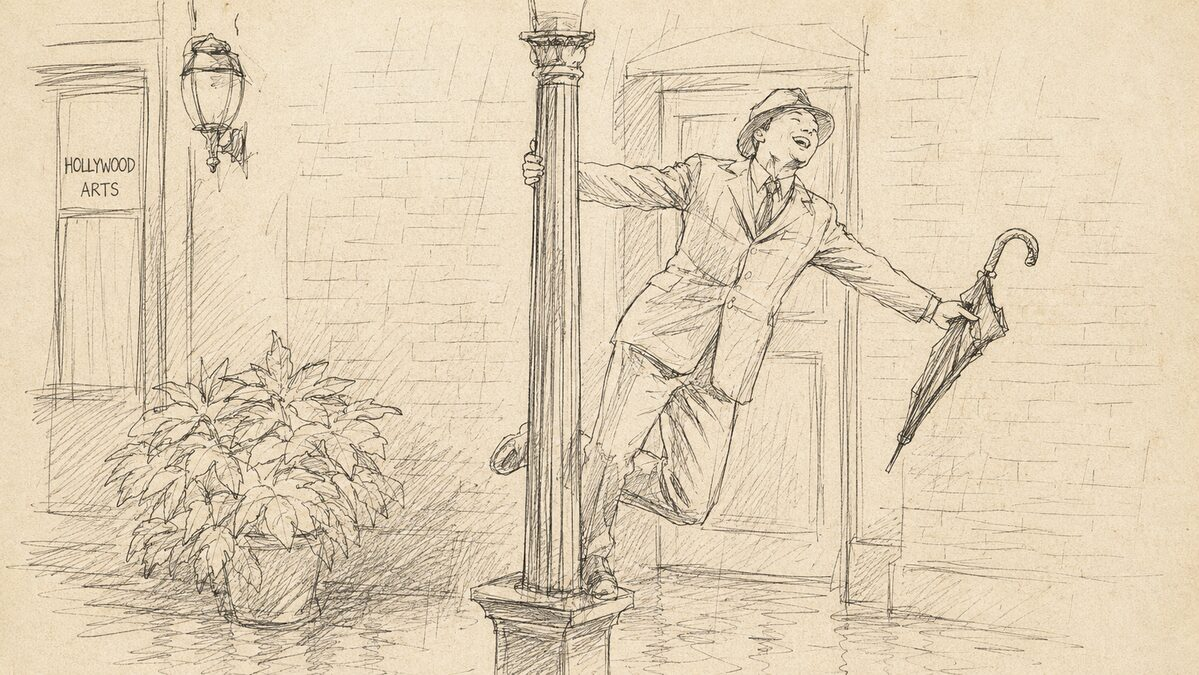
\includegraphics[width=0.92\textwidth,height=0.76\textheight,keepaspectratio]{sing.jpg}
    \end{center}
\end{frame}

%%%%%%%%%%%%%%%%%%%%%%%%%%%%%%%%%%%%%%%%%%%%%%%%%%

\begin{frame}[plain]
    \vspace{-0.5mm}
    \begin{center}
        \large\bfseries welcome to the world of
        
\begin{tikzpicture}[baseline=(ain.base)]
            \node[inner sep=0pt, outer sep=0pt, anchor=base east] (p) at (0,0) {P};
            \draw[red, line width=1.1pt] (p.south west) -- (p.north east);
            \node[red, inner sep=0pt, outer sep=0pt, yshift=0.65ex] at (p.center) {R};
            \node[inner sep=0pt, outer sep=0pt, anchor=base west] (ain) at (0,0) {AIN};
        \end{tikzpicture}
    \end{center}
    \vspace{1mm}

    \centering
    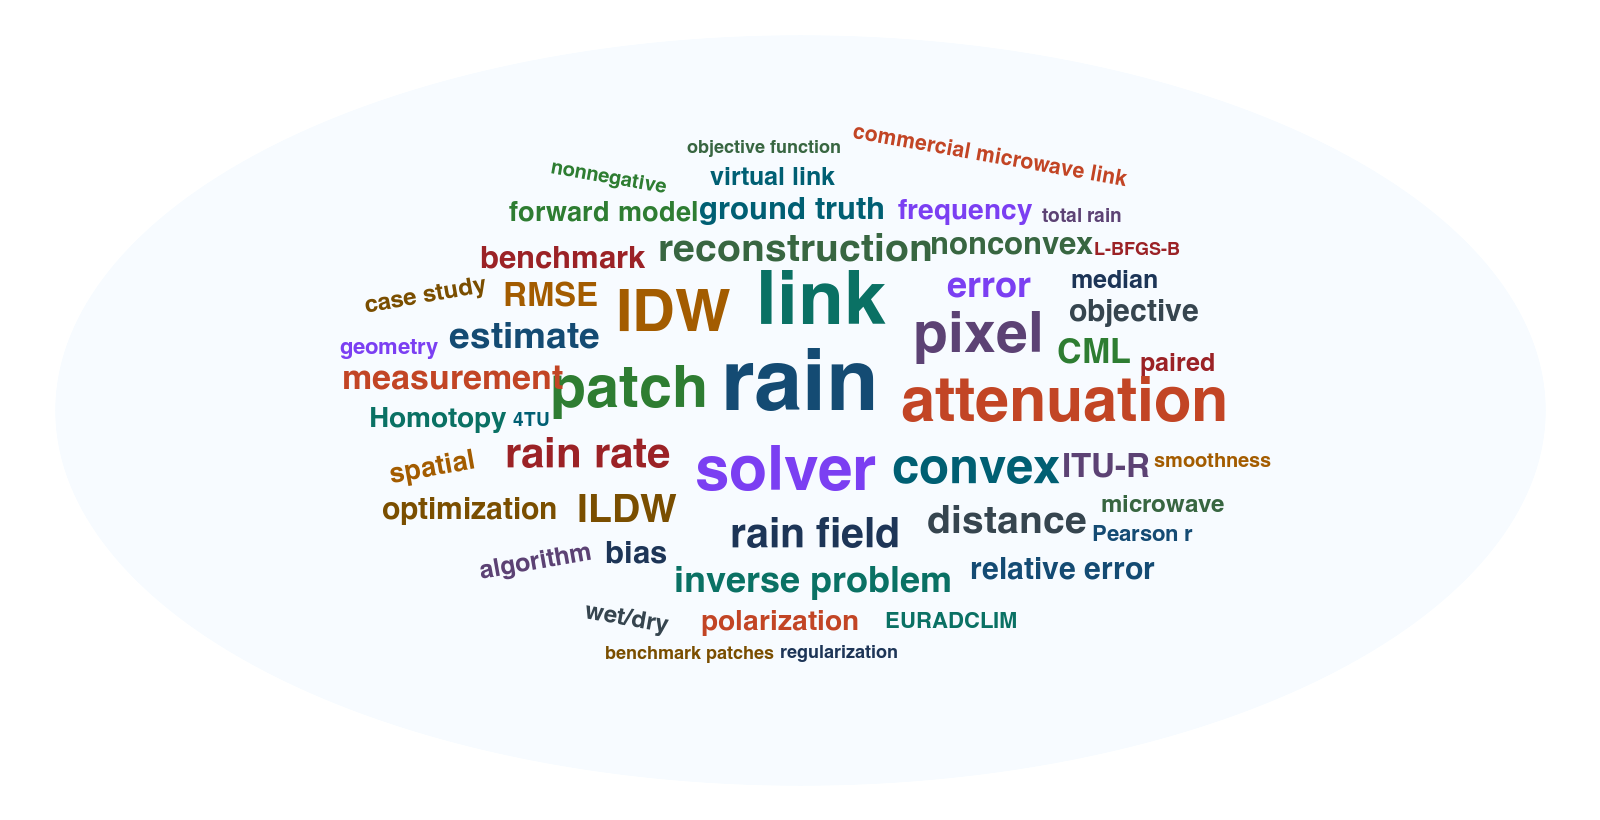
\includegraphics[width=0.98\textwidth,height=0.80\textheight,keepaspectratio]{word-cloud.png}
\end{frame}

%%%%%%%%%%%%%%%%%%%%%%%%%%%%%%%%%%%%%%%%%%%%%%%%%%

\begin{frame}[plain]
    \vspace{-0.5mm}
    \begin{center}\large\bfseries Glossary: Microwave Links\end{center}
    \vspace{4mm}

    \textbf{Commercial microwave link (CML).}

    \vspace{1mm}
    A wireless connection between two antennas. Such links are used in 5G backhaul networks. In this talk, a link is represented by a line segment $\ell$.

    \vspace{3mm}
    \textbf{Frequency.}

    \vspace{1mm}
    The carrier frequency of the microwave signal.

    \vspace{3mm}
    \textbf{Polarization.}

    \vspace{1mm}
    The orientation of the electric field of the microwave signal.
\end{frame}



%%%%%%%%%%%%%%%%%%%%%%%%%%%%%%%%%%%%%%%%%%%%%%%%%%

\begin{frame}[plain]
    \vspace{-0.5mm}
    \begin{center}\large\bfseries Glossary: Rain Field and Attenuation\end{center}
    \vspace{4mm}

    \vspace{3mm}
    \textbf{Rain field.}

    \vspace{1mm}
    A function from a rectangular geographic area $\Omega$ to non-negative real values:
    \[
        R:\Omega \to \mathbb{R}_{\ge 0}.
    \]
    For a pixel $s\in\Omega$, $R(s)$ is the rain rate at that pixel, measured in mm/h.

    \vspace{3mm}
    \textbf{Attenuation.}

    \vspace{1mm}
    Water molecules are electric dipoles, so raindrops interact with the microwave signal, as in a microwave oven. This weakens the signal and reduces the received signal power.
\end{frame}

%%%%%%%%%%%%%%%%%%%%%%%%%%%%%%%%%%%%%%%%%%%%%%%%%%

\begin{frame}[plain]
    \vspace{-0.5mm}
    \begin{center}\large\bfseries Glossary: Forward Model\end{center}
    \vspace{4mm}

    \textbf{Forward model.}

    \vspace{1mm}
    A known function that maps the hidden object to the measurements:
    \[
        \text{object} \longrightarrow \text{measurements}.
    \]

    \vspace{3mm}
    \textbf{In our case.}

    \vspace{1mm}
    The hidden object is the rain field $R$, and the measurements are the link attenuations:
    \[
        R \longrightarrow \{A_\ell\}_\ell .
    \]

\end{frame}

%%%%%%%%%%%%%%%%%%%%%%%%%%%%%%%%%%%%%%%%%%%%%%%%%%

\begin{frame}[plain]
    \vspace{-0.5mm}
    \begin{center}\large\bfseries Glossary: Inverse Problem\end{center}
    \vspace{4mm}

    \textbf{Inverse problem.}

    \vspace{1mm}
    Recover the hidden object from the measurements:
    \[
        \text{measurements} \longrightarrow \text{estimated object}.
    \]

    \vspace{3mm}
    \textbf{In our case.}

    \vspace{1mm}
    Given the link attenuations, estimate the rain field:
    \[
        \{A_\ell\}_\ell \longrightarrow \hat R .
    \]

    \vspace{3mm}
    \textbf{Ground truth and reconstruction.}

    \vspace{1mm}
    The true rain field is denoted by $R$. An algorithm returns an estimated rain field $\hat R$.
\end{frame}
%%%%%%%%%%%%%%%%%%%%%%%%%%%%%%%%%%%%%%%%%%%%%%%%%%

\begin{frame}[plain]
    \vspace{-0.5mm}
    \begin{center}\large\bfseries Glossary: Evaluation Metrics\end{center}
    \vspace{3mm}

    Let $R_i$ be the ground-truth rain rate at pixel $i$, and let $\hat R_i$ be the estimated rain rate.

    \[
        \mathrm{Bias}
        =
        \frac{1}{n}\sum_{i=1}^n(\hat R_i-R_i) \quad \text{{\footnotesize the sample mean of the error $e_i=\hat R_i-R_i$.}}
    \]



    \[
        \mathrm{RMSE}
        =
        \sqrt{\frac{1}{n}\sum_{i=1}^n(\hat R_i-R_i)^2} \quad \text{{\footnotesize standard deviation of the error if the bias is zero}}
    \]




    \vspace{2mm}
    \textbf{Pearson correlation.}   covariance of the standardized variables = cosine of angle between $R$ and $\hat{R}$.
    \[
        r
        =
        \frac{\sum_i(\hat R_i-\bar{\hat R})(R_i-\bar R)}
        {\sqrt{\sum_i(\hat R_i-\bar{\hat R})^2}
            \sqrt{\sum_i(R_i-\bar R)^2}}
    \]

\end{frame}
%%%%%%%%%%%%%%%%%%%%%%%%%%%%%%%%%%%%%%%%%%%%%%%%%%

\begin{frame}[plain]
    \vspace{-0.5mm}
    \begin{center}\Large\bfseries append slide saying, now i can present my EGU slides. add a funny image with a relief from a pain\end{center}
    \vspace{3mm}

    \centering
    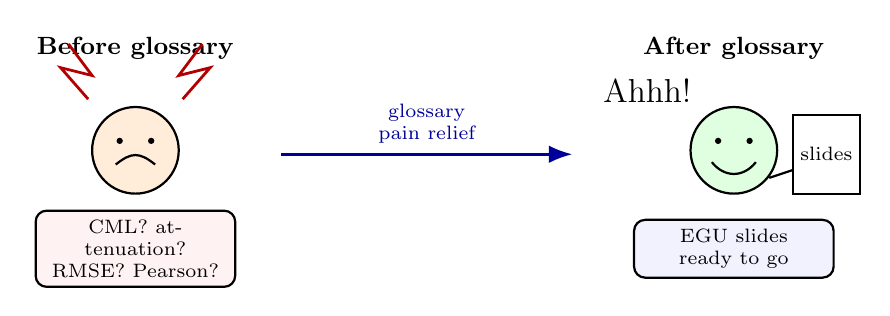
\begin{tikzpicture}[line width=0.8pt, font=\small]
        % Before glossary: terminology headache.
        \node[align=center] at (-4.2,2.1) {\textbf{Before glossary}};
        \draw[fill=orange!15] (-4.2,0.8) circle (0.55);
        \fill (-4.4,0.92) circle (0.04);
        \fill (-4.0,0.92) circle (0.04);
        \draw (-4.45,0.62) .. controls (-4.25,0.78) and (-4.15,0.78) .. (-3.95,0.62);
        \draw[red!70!black, line width=1pt] (-4.8,1.45) -- (-5.15,1.85) -- (-4.75,1.75) -- (-5.05,2.15);
        \draw[red!70!black, line width=1pt] (-3.6,1.45) -- (-3.25,1.85) -- (-3.65,1.75) -- (-3.35,2.15);
        \node[draw, rounded corners, fill=red!5, align=center, font=\scriptsize, text width=2.3cm]
        at (-4.2,-0.45) {CML? attenuation?\\RMSE? Pearson?};

        % Transition arrow.
        \draw[-{Latex[length=3mm]}, line width=1.0pt, blue!60!black]
        (-2.35,0.75) -- (1.35,0.75)
        node[midway, above, align=center, font=\scriptsize] {glossary\\pain relief};

        % After glossary: relaxed presenter.
        \node[align=center] at (3.4,2.1) {\textbf{After glossary}};
        \draw[fill=green!12] (3.4,0.8) circle (0.55);
        \fill (3.2,0.92) circle (0.04);
        \fill (3.6,0.92) circle (0.04);
        \draw (3.12,0.65) .. controls (3.28,0.45) and (3.52,0.45) .. (3.68,0.65);
        \node[draw, rounded corners, fill=blue!5, align=center, font=\scriptsize, text width=2.3cm]
        at (3.4,-0.45) {EGU slides\\ready to go};
        \draw[fill=white] (4.15,0.25) rectangle (5.0,1.25);
        \node[font=\scriptsize, align=center] at (4.575,0.75) {slides};
        \draw (3.85,0.45) -- (4.15,0.55);
        \node[font=\large] at (2.3,1.55) {Ahhh!};
    \end{tikzpicture}
\end{frame}

%%%%%%%%%%%%%%%%%%%%%%%%%%%%%%%%%%%%%%%%%%%%%%%%%%

\begin{frame}[plain]
    \begin{tikzpicture}[remember picture,overlay]
        \node[anchor=center,inner sep=0pt,xshift=0.185\paperwidth,yshift=-0.085\paperheight]
        at (current page.north west)
        {
\includegraphics[height=0.105\paperheight]{logos/MPI.png}};
        \node[anchor=center,inner sep=0pt,yshift=-0.085\paperheight]
        at (current page.north)
        {
\includegraphics[height=0.105\paperheight,trim=255bp 236bp 232bp 169bp,clip]{logos/TAU-LOGO-Eng_BW.pdf}};
        \node[anchor=center,inner sep=0pt,xshift=-0.185\paperwidth,yshift=-0.085\paperheight]
        at (current page.north east)
        {
\includegraphics[height=0.105\paperheight,trim=132bp 125bp 127bp 123bp,clip]{logos/university-of-cologne-logo.jpg}};
    \end{tikzpicture}
    \vspace{0.255\paperheight}
    \begin{center}
        {\Large\bfseries \inserttitle\par}
        \vspace{5mm}
        {\normalsize \insertauthor\par}
        \vspace{2mm}
        {\small \insertinstitute\par}
        \vspace{5mm}
        {\small \insertdate\par}
    \end{center}
\end{frame}



\begin{frame}[plain]
    \vspace{-0.5mm}
    \begin{center}\large\bfseries Estimate Rainfall Field from Microwave Link Attenuation\end{center}
    \vspace{1mm}

    \begin{columns}[T,totalwidth=\textwidth]
        \begin{column}{0.59\textwidth}
            \small
            \textbf{Opportunity.}

            \vspace{1mm}
            Rain attenuates 5G microwave backhaul links.

            \vspace{3mm}
            \textbf{Forward model.}

            \vspace{1mm}
            For rain field $R$ and link $\ell$, ITU-R rain-attenuation model:
            \[
                A_\ell = \int_\ell \kappa R(s)^\alpha\,ds,
            \]
            where $\kappa$ and $\alpha$ depend on the link frequency and polarization.

            \vspace{3mm}
            \textbf{Inverse problem.}

            \vspace{1mm}
            Given link attenuations $\{A_\ell\}$, recover the spatial rainfall field $R$.
        \end{column}
        \begin{column}{0.36\textwidth}
            \centering
            \vspace{-0.3cm}
            {\tiny 4TU CML Overeem et al. (2016)}

            \vspace{0.5mm}
            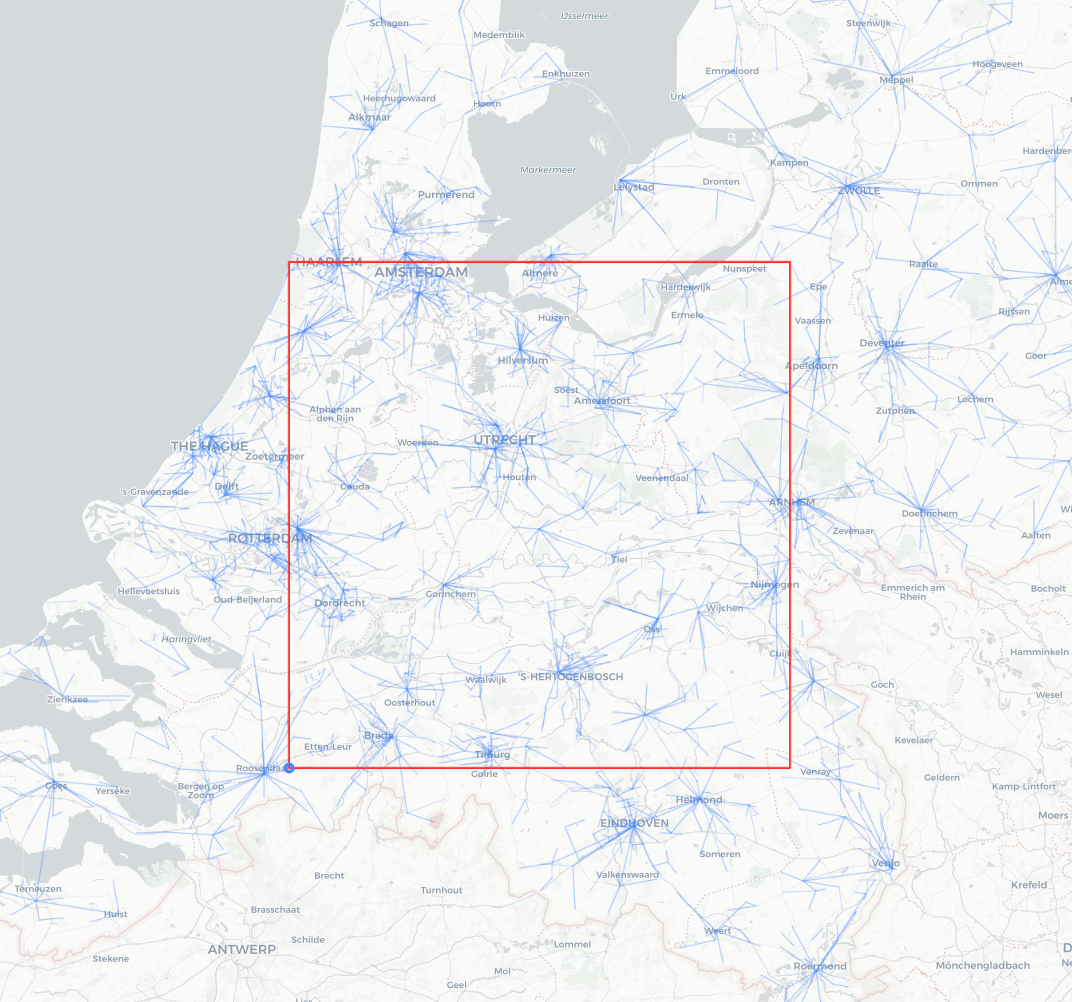
\includegraphics[height=0.21\textheight,keepaspectratio,trim={405bp 400bp 345bp 330bp},clip]{map-4TU-Links.png}

            \vspace{2mm}
            {\tiny ITU-R P.838-3, horizontal polarization}

            \vspace{0.5mm}
            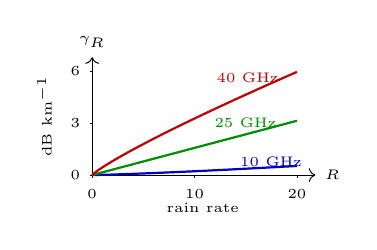
\begin{tikzpicture}[x=0.13cm,y=0.22cm,font=\tiny]
                \draw[->,line width=0.35pt] (0,0) -- (21.8,0) node[right] {$R$};
                \draw[->,line width=0.35pt] (0,0) -- (0,6.8) node[above] {$\gamma_R$};
                \foreach \x/\lab in {0/0,10/10,20/20}
                \draw[line width=0.25pt] (\x,0) -- (\x,-0.15) node[below=1pt] {\lab};
                \foreach \y/\lab in {0/0,3/3,6/6}
                \draw[line width=0.25pt] (0,\y) -- (-0.25,\y) node[left] {\lab};
                \draw[blue!75!black,line width=0.8pt]
                (0,0) -- plot[domain=0.05:20,samples=80] (\x,{0.01217*pow(\x,1.257)});
                \draw[green!55!black,line width=0.8pt]
                (0,0) -- plot[domain=0.05:20,samples=80] (\x,{0.1571*pow(\x,0.9991)});
                \draw[red!75!black,line width=0.8pt]
                (0,0) -- plot[domain=0.05:20,samples=80] (\x,{0.4431*pow(\x,0.8673)});
                \node[blue!75!black,anchor=west] at (13.5,0.75) {$10$ GHz};
                \node[green!55!black,anchor=west] at (11.0,3.0) {$25$ GHz};
                \node[red!75!black,anchor=west] at (11.2,5.6) {$40$ GHz};
                \node[anchor=north] at (10.8,-1.05) {rain rate};
                \node[anchor=south,rotate=90] at (-3.0,3.4) {dB km$^{-1}$};
            \end{tikzpicture}

            \vspace{-0.3cm}
            {\tiny Rain field}

            \vspace{0.5mm}
            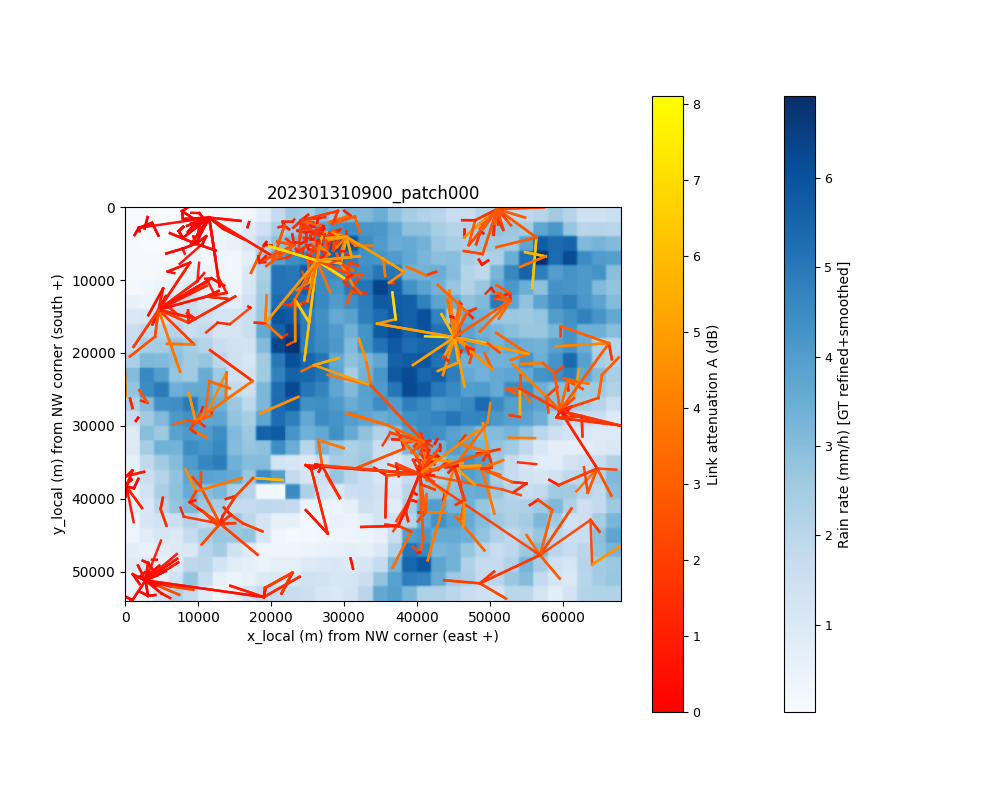
\includegraphics[height=0.25\textheight,keepaspectratio,trim={94bp 142bp 350bp 178bp},clip]{0900_patch000.png}

        \end{column}
    \end{columns}

    \begin{tikzpicture}[remember picture,overlay]
        \node[anchor=south west, text width=0.56\paperwidth,
            font=\fontsize{4.5}{5}\selectfont, align=left]
        at ([xshift=4mm,yshift=6mm]current page.south west)
        {Rain attenuation and CML rainfall sensing: Gunn and East (1954), Olsen et al. (1978), ITU-R P.838-3, Messer et al. (2006), Overeem et al. (2013), Fencl (2015), Chwala and Kunstmann (2019), Graf et al. (2020), Blettner et al. (2023).};
    \end{tikzpicture}
\end{frame}

%%%%%%%%%%%%%%%%%%%%%%%%%%%%%%%%%%%%%%%%%%%%%%%%%%
\begin{frame}[plain]
    \vspace{-0.5mm}
    \begin{center}\large\bfseries Methodology\end{center}
    \vspace{5mm}

    \textbf{Benchmark construction.}

    \vspace{1mm}
    We build a noise-free benchmark of $100$ rain scenarios. Each scenario contains:
    \begin{itemize}
        \item a ground-truth rainfall field,
        \item link attenuations computed from the ITU-R forward model.
    \end{itemize}

    \vspace{3mm}
    \textbf{Inverse solvers.}

    \vspace{1mm}
    We develop new inverse solvers for estimating rainfall fields from link attenuations.

    \vspace{3mm}
    \textbf{Baselines and evaluation.}

    \vspace{1mm}
    We compare against inverse distance weighting (IDW), a common virtual-gauge interpolation baseline in CML rainfall mapping.

    \vfill
    {\tiny Benchmark sources: EURADCLIM, Overeem et al. (2023). 4TU CML data, Overeem et al. (2016). \\
        CML interpolation baselines: Rayitsfeld et al. (2012), Blettner et al. (2023), Overeem et al. (2016), Chwala and Kunstmann (2019), Eshel et al. (2020, 2021).}
\end{frame}
%%%%%%%%%%%%%%%%%%%%%%%%%%%%%%%%%%%%%%%%%%%%%%%%%%

{
    \usebackgroundtemplate{}
    \setbeamertemplate{headline}{}
    \setbeamertemplate{footline}{}
    \begin{frame}[plain]
        \vspace{-0.5mm}
        \begin{center}\large\bfseries Benchmark Construction\end{center}
        \vspace{-2mm}
        \centering
        \resizebox{0.985\textwidth}{0.84\textheight}{% TikZ content only. Intended to be included from benchmark-construction-slide.tex.
\begin{tikzpicture}[
  x=1cm,
  y=1cm,
  image/.style={inner sep=0pt},
  sidecaption/.style={font=\scriptsize\bfseries, align=center, text=black},
  note/.style={font=\tiny, align=center, text=black!70},
  flow/.style={-{Latex[length=2.3mm]}, line width=0.85pt, draw=blue!65!black},
  softflow/.style={-{Latex[length=2.2mm]}, line width=0.75pt, draw=blue!45!black},
]

% 2 x 2 layout:
% NW: EURADCLIM, NE: 100 patch locations, SW: 4TU, SE: example patch.
% All raster panels are intentionally forced to roughly the same square size.

\newcommand{\panelsize}{3.25cm}
\newcommand{\patchsize}{3.65cm}

\node[image] (eurad) at (2.45,4.85)
  {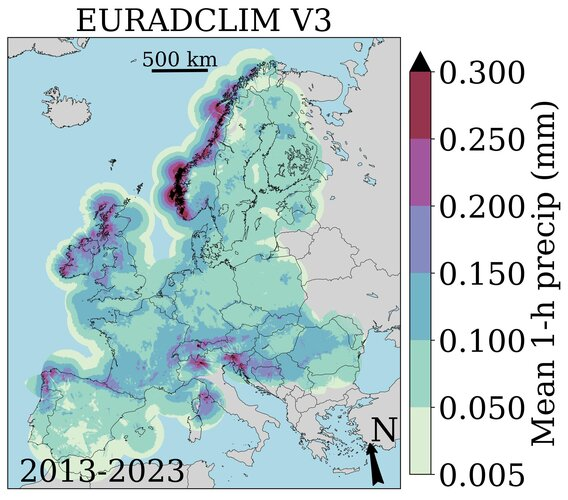
\includegraphics[width=\panelsize,height=\panelsize]{EURADCLIM.jpg}};
\node[sidecaption, anchor=north west] at ([xshift=8mm,yshift=-1mm]eurad.north)
  {\textsuperscript{*}};

\node[image] (locations) at (9.00,4.85)
  {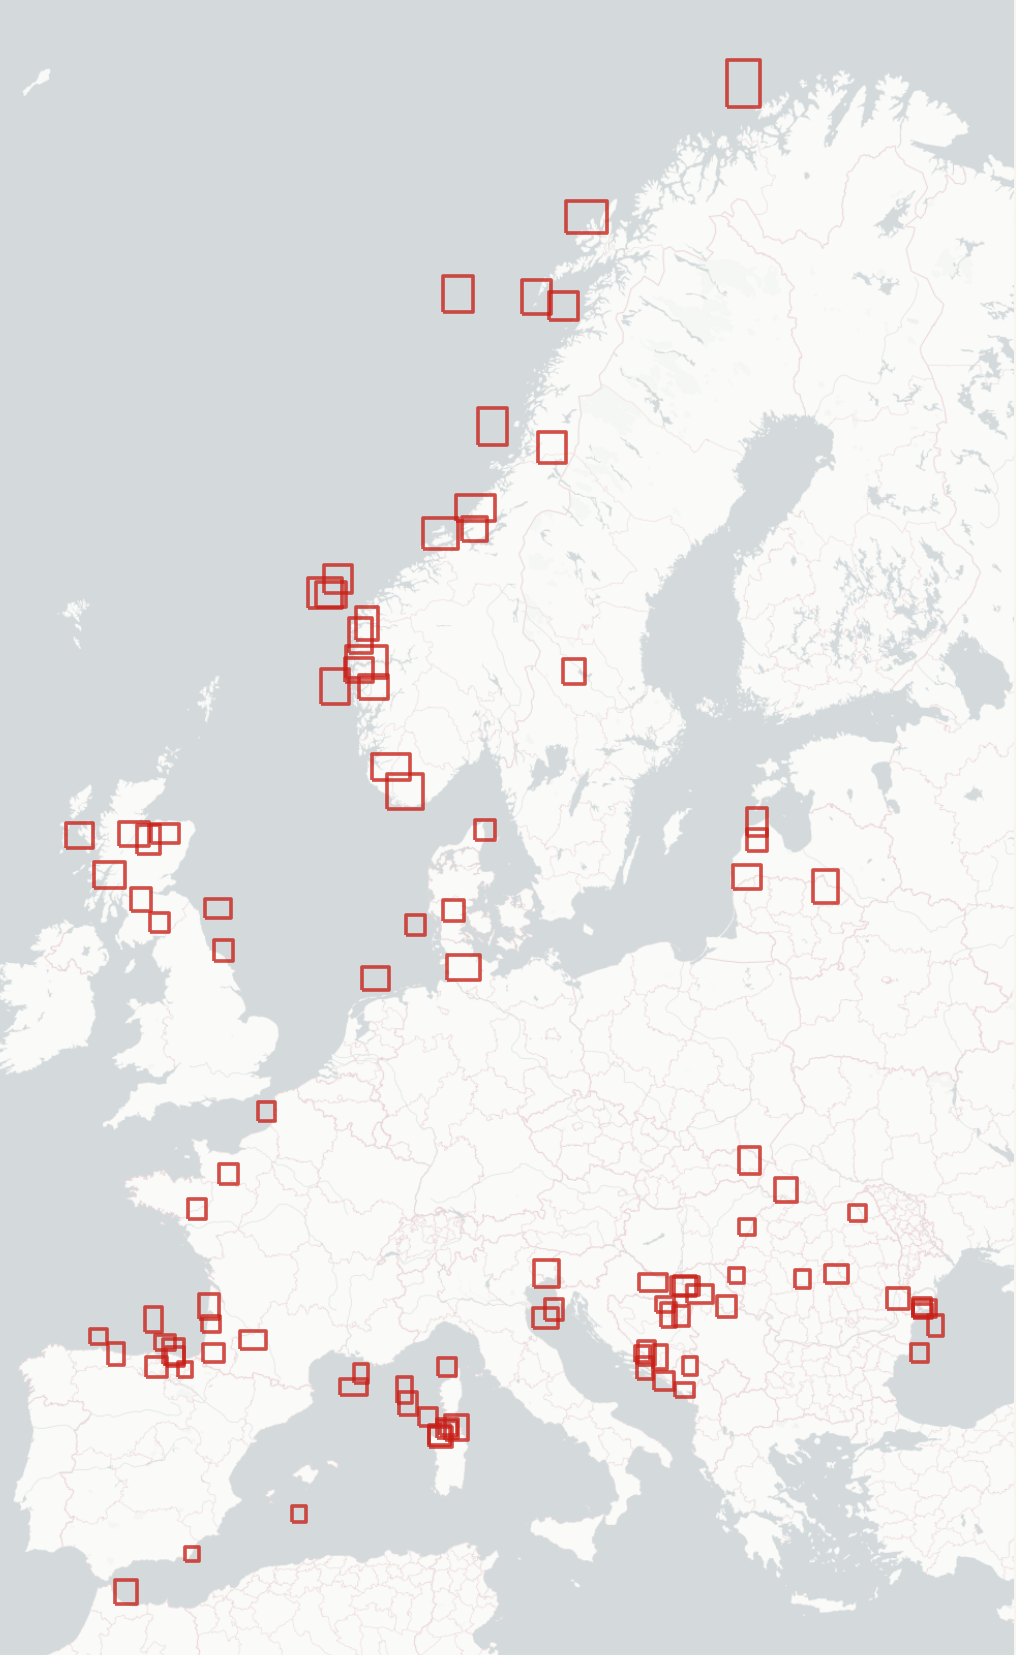
\includegraphics[width=\panelsize,height=\panelsize]{100patches-locations.png}};

\node[image] (links) at (2.45,1.10)
  {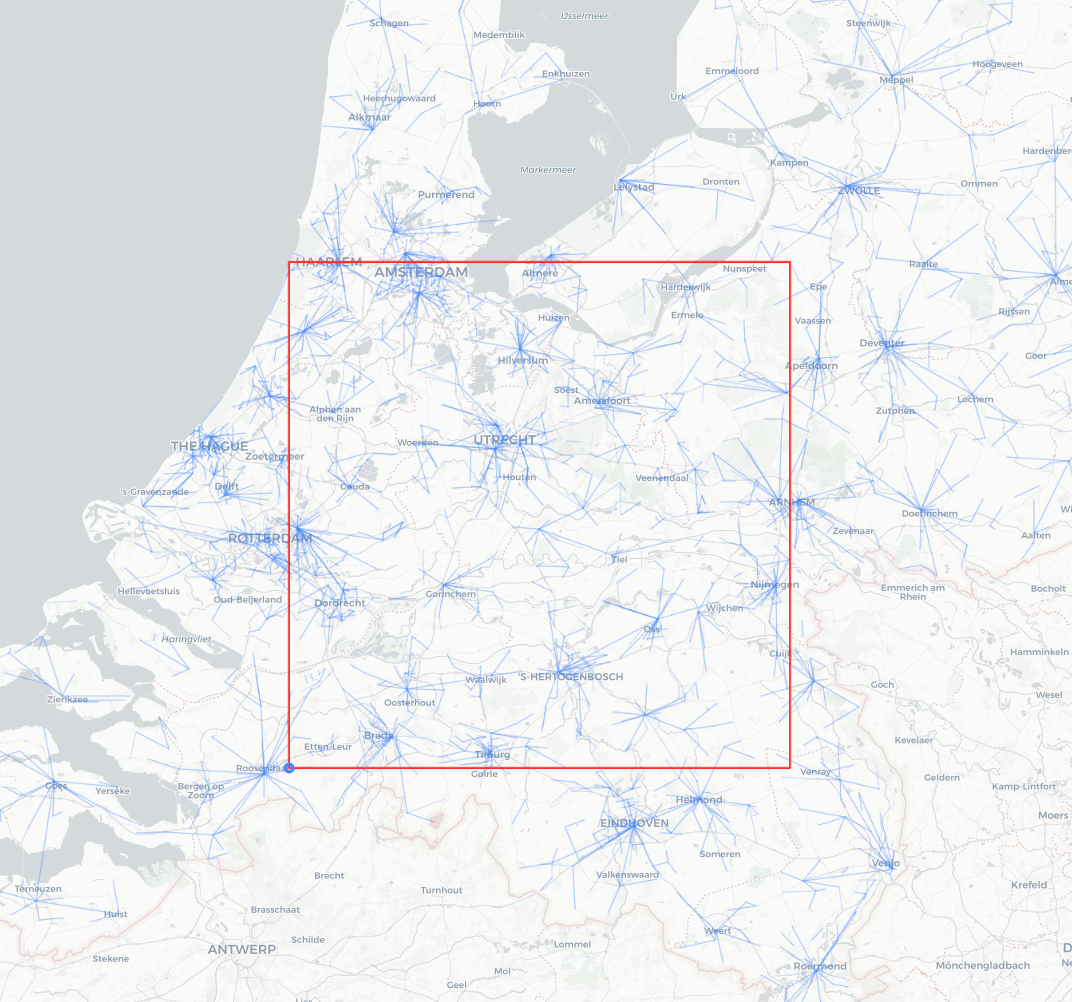
\includegraphics[width=\panelsize,height=\panelsize,trim={248bp 194bp 242bp 223bp},clip]{map-4TU-Links.png}};
\node[sidecaption, anchor=north] at ([yshift=-1mm]links.north)
  {4TU\textsuperscript{\ensuremath{\dagger}}};

% Keep the original top-left corner of the example patch while enlarging it.
\node[image, anchor=north west] (patch) at (7.175,2.725)
  {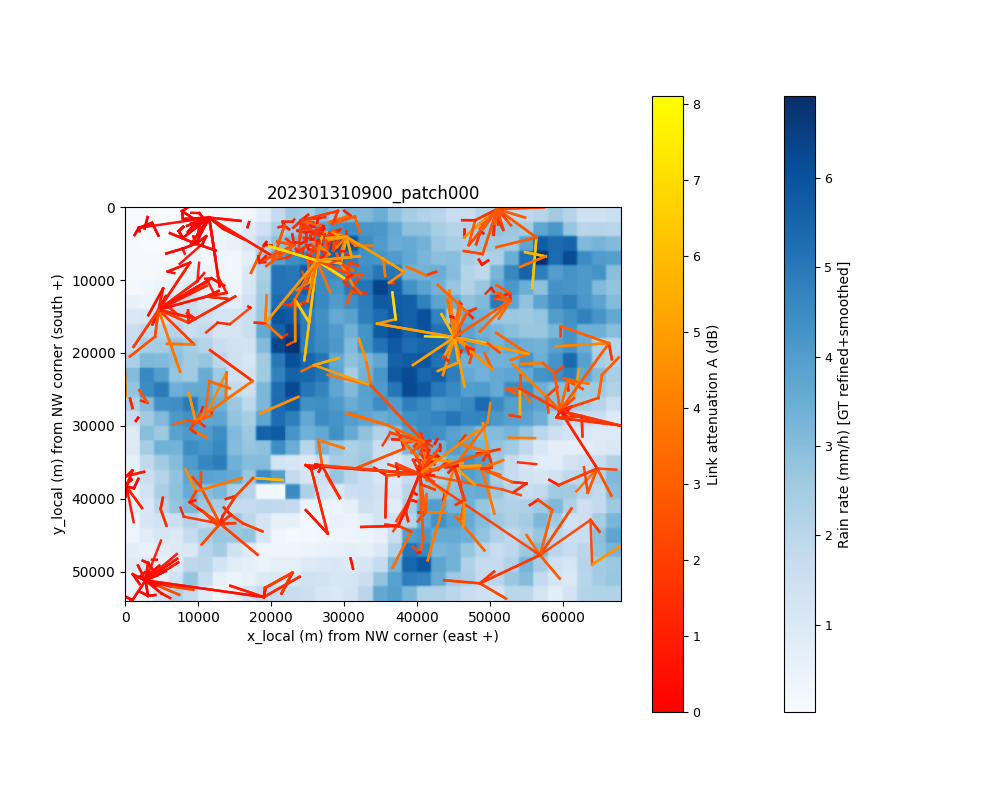
\includegraphics[width=\patchsize,height=\patchsize]{0900_patch000.png}};

% Axis-parallel arrows, each with a single straight segment.
\draw[flow]
  (eurad.east) -- node[note, above, midway] {automatic extraction\\of rain event}
  (locations.west);

\draw[flow]
  (locations.south) -- node[note, left=1.5mm, midway, anchor=east, align=center] {link atten\\=\\ITU(rain)}
  ([yshift=-6mm]patch.north);

\draw[softflow]
  (links.east |- patch.west) -- node[note, above, midway] {clip link geometry\\+ parameters}
  (patch.west);

% Source line inside the slide canvas, not as a Beamer footer.
\node[anchor=south west, font=\fontsize{4.5}{4.8}\selectfont, text=black!65, align=left] at (0.0,-1.05)
  {\textsuperscript{*} EURADCLIM rainfall fields: Overeem et al. (2023), KNMI.};
\node[anchor=south east, font=\fontsize{4.5}{4.8}\selectfont, text=black!65, align=right] at (11.2,-1.05)
  {\textsuperscript{\ensuremath{\dagger}} CML data: Overeem et al. (2016), 4TU.ResearchData. Attenuation: ITU-R P.838-3.};

\end{tikzpicture}
}
    \end{frame}
}

%%%%%%%%%%%%%%%%%%%%%%%%%%%%%%%%%%%%%%%%%%%%%%%%%%

\begin{frame}[plain]
    \vspace{-0.5mm}
    \begin{center}\large\bfseries New Inverse Solvers\end{center}
    \vspace{5mm}

    \renewcommand{\arraystretch}{1.45}
    \begin{tabular}{p{0.25\textwidth}p{0.67\textwidth}}
        \textbf{Technique}                   & \textbf{Main idea}                                              \\
        \hline
        IDW standard                         &
        Inverse distance weighting (IDW) using distance to the link midpoint, treated as a virtual rain gauge. \\
        ILDW                                 &
        Inverse link-distance weighting using distance to the link segment.                                    \\
        Constrained regularized optimization &
        Estimate a non-negative rain field by minimizing attenuation mismatch
        $(\hat A_\ell-A_\ell)^2$, first- and second-derivative penalties, and total rain.                      \\
    \end{tabular}

    \vfill
    {\tiny Virtual-gauge and IDW-based CML reconstruction: Rayitsfeld et al. (2012), Overeem et al. (2013, 2016), Chwala and Kunstmann (2019), Eshel et al. (2020, 2021), Blettner et al. (2023).}
\end{frame}

%%%%%%%%%%%%%%%%%%%%%%%%%%%%%%%%%%%%%%%%%%%%%%%%%%

\begin{frame}[plain]
    \vspace{-0.5mm}
    \begin{center}\large\bfseries
        Problem: Nonconvex objective
    \end{center}
    \vspace{4mm}

    Attenuation mismatch objective
    $
        \sum_{\ell}
        \bigl(\hat A_\ell(\hat R)-A_\ell\bigr)^2
    $
    \textbf{not convex} in the rain field if $\alpha_\ell\neq 1$.

    \vspace{3mm}
    \begin{columns}[T,totalwidth=\textwidth]
        \begin{column}{0.56\textwidth}
            \textbf{Consequence.}
            \begin{itemize}
                \item Solver might converge to a local solution.
                \item The result can depend on the initial rain field.
            \end{itemize}
        \end{column}
        \begin{column}{0.36\textwidth}
            \centering
            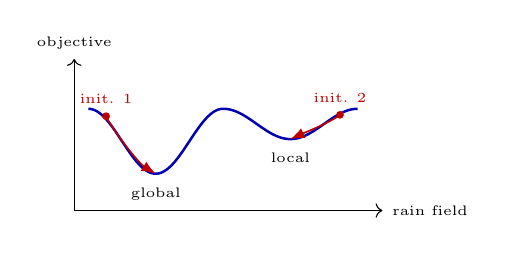
\begin{tikzpicture}[x=0.9cm,y=0.55cm,font=\tiny]
                \draw[->,line width=0.4pt] (-2.0,0) -- (2.35,0) node[right] {rain field};
                \draw[->,line width=0.4pt] (-2.0,0) -- (-2.0,3.5) node[above] {objective};
                \draw[blue!70!black,line width=0.9pt,smooth,domain=90:450,samples=90]
                plot({-1.8 + (\x-90)/360*1.9},{2.35 + 0.75*(sin(\x)-1)});
                \draw[blue!70!black,line width=0.9pt,smooth,domain=90:450,samples=90]
                plot({0.1 + (\x-90)/360*1.9},{2.35 + 0.35*(sin(\x)-1)});
                \fill[red!75!black] (-1.55,2.18) circle (1.4pt);
                \fill[red!75!black] (1.75,2.21) circle (1.4pt);
                \draw[-{Latex[length=1.8mm]},red!75!black,line width=0.6pt]
                (-1.55,2.16) .. controls (-1.28,1.45) and (-1.05,1.05) .. (-0.85,0.85);
                \draw[-{Latex[length=1.8mm]},red!75!black,line width=0.6pt]
                (1.75,2.20) .. controls (1.50,1.95) and (1.25,1.8) .. (1.05,1.65);
                \node[red!75!black,anchor=south] at (-1.55,2.24) {init. 1};
                \node[red!75!black,anchor=south] at (1.75,2.28) {init. 2};
                \node[anchor=north] at (-0.85,0.75) {global};
                \node[anchor=north] at (1.05,1.55) {local};
            \end{tikzpicture}
        \end{column}
    \end{columns}
\end{frame}

%%%%%%%%%%%%%%%%%%%%%%%%%%%%%%%%%%%%%%%%%%%%%%%%%%

\begin{frame}[plain]
    \vspace{-0.5mm}
    \begin{center}\large\bfseries Convex Surrogate for Constrained Regularized Optimization
    \end{center}
    \vspace{4mm}

    At $f_0 \approx 25$ GHz for horizontal polarization, the ITU-R exponent satisfies
    $\alpha_0 \approx 1$. Then the forward map is linear in the rain field:
    \[
        \tikz[remember picture,baseline=(hatAzero.base)]
        \node[inner sep=0pt] (hatAzero) {$\hat A^0_\ell(\hat R)$};
        =
        \int_\ell \kappa_0 \hat R(s)\,ds .
    \]
    \begin{tikzpicture}[remember picture,overlay]
        \node[draw=blue!60!black, fill=blue!5, rounded corners,
            font=\scriptsize, align=center, inner sep=2pt,
            anchor=east,
            at={([xshift=-7mm,yshift=-4mm]hatAzero.west)}] (linbubble)
        {linear in $\hat{R}$};
        \draw[-{Latex[length=1.8mm]}, blue!60!black, line width=0.55pt]
        (linbubble.east) .. controls ([xshift=8mm,yshift=2mm]linbubble.east)
        and ([xshift=-8mm,yshift=-5mm]hatAzero.south west) .. (hatAzero.south west);
    \end{tikzpicture}

    \vspace{2mm}
    \textbf{Replace each link by a virtual link at $f_0$.}
    Keep the same geometry and the same rain-equivalent value:
    \[
        R_\ell
        =
        \left(
        \frac{A_\ell/|\ell|}{\kappa_\ell}
        \right)^{1/\alpha_\ell},
        \qquad
        A^0_\ell
        =
        \kappa_0 R_\ell |\ell| .
    \]

    \vspace{2mm}
    The attenuation term becomes a convex least-squares term:
    \[
        \sum_\ell
        \bigl(\hat A^0_\ell(\hat R)-A^0_\ell\bigr)^2 .
    \]

\end{frame}

%%%%%%%%%%%%%%%%%%%%%%%%%%%%%%%%%%%%%%%%%%%%%%%%%%
\begin{frame}[plain]
    \vspace{5mm}
    \begin{center}\large\bfseries Results\end{center}
    \vspace{1mm}

    \centering
    \renewcommand{\arraystretch}{1.12}
    \setlength{\tabcolsep}{7pt}
    \begin{tabular}{lccc}
        \hline
        \textbf{Method} & \textbf{Avg. RMSE} & \textbf{Avg. $|\mathrm{Bias}|$} & \textbf{Avg. Pearson $r$} \\
        \hline
        IDW             & $1.31$             & $0.16$                          & $0.87$                    \\
        ILDW            & $1.24$             & $0.14$                          & $0.89$                    \\
        Convex Solver   & $\mathbf{0.85}$    & $\mathbf{0.05}$                 & $\mathbf{0.95}$           \\
        \hline
    \end{tabular}
    \par\vskip 3mm
    \noindent\hspace*{-20mm}%
    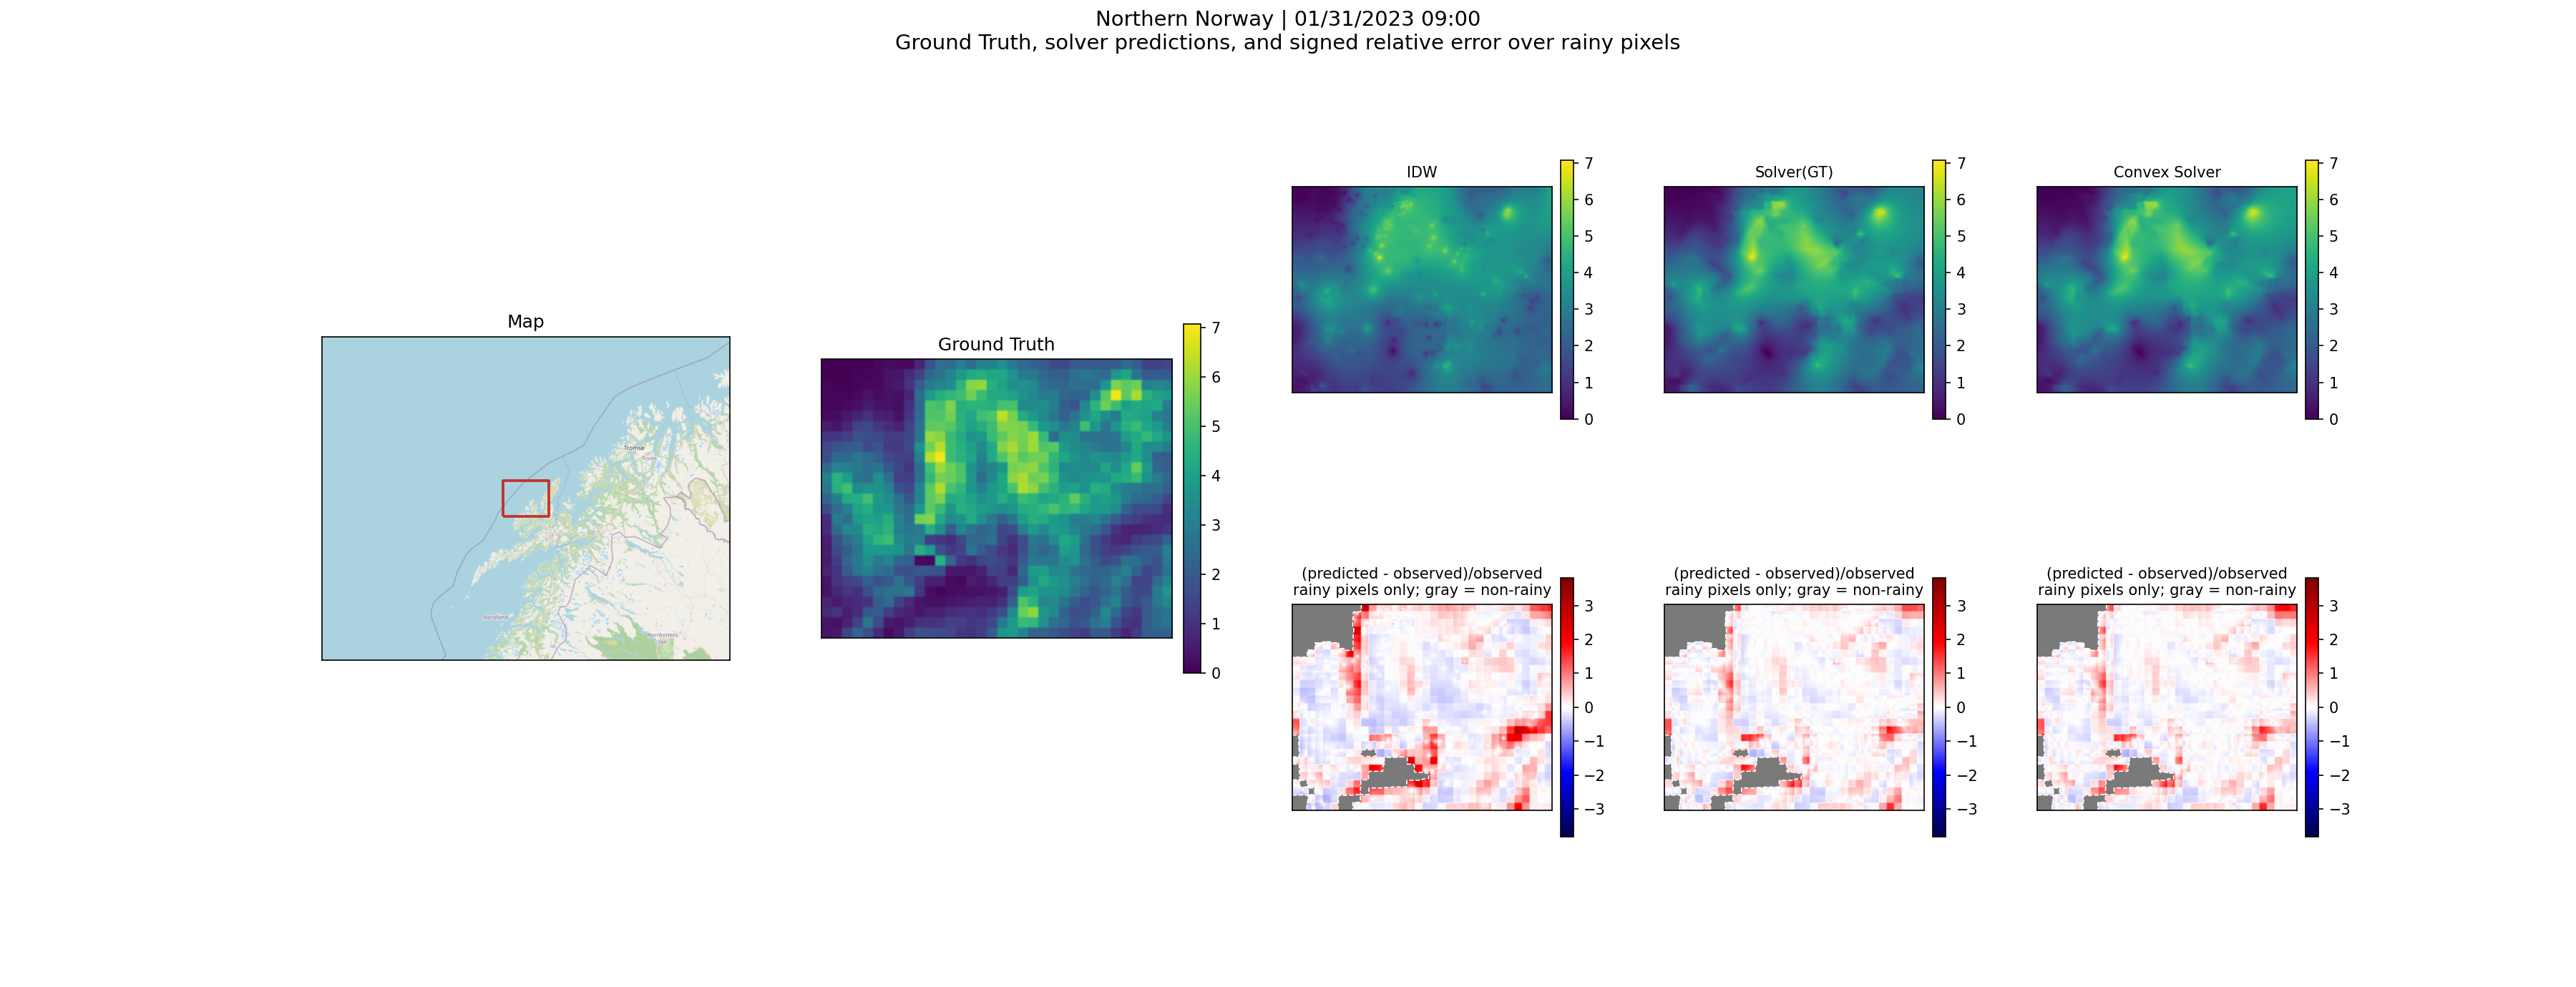
\includegraphics[
        width=1.2\textwidth,
        keepaspectratio,
        trim={0bp 0bp 0bp 95bp},
        clip
    ]{../images/case_studies/new_pattern_one/RAD_OPERA_HOURLY_RAINFALL_ACCUMULATION_202301310900_patch000.png}

\end{frame}

%%%%%%%%%%%%%%%%%%%%%%%%%%%%%%%%%%%%%%%%%%%%%%%%%%
\begin{frame}[plain]
    \begin{tikzpicture}[remember picture,overlay]
        \fill[white] (current page.south west) rectangle (current page.north east);

        % Square poster area, scaled to fit the 16:9 slide height.
        \begin{scope}[shift={(current page.center)},scale=0.75,x=1mm,y=1mm]
            % Blue block text, in the spirit of the Miles Davis poster.
            \node[anchor=west,text=blue!70!black,
                font=\fontsize{58}{53}\selectfont\bfseries]
            at (5,15) {SO};
            \node[anchor=west,text=blue!70!black,
                font=\fontsize{58}{53}\selectfont\bfseries]
            at (-17,-9) {WHAT ?};

            % Minimal black trumpet-player silhouette.
            \coordinate (hip) at (-36,-15);
            \coordinate (shoulder) at (-44,18);
            \coordinate (head) at (-42,28);

            % Body and head.
            \fill[black]
            ([xshift=-4mm,yshift=-23mm]hip)
            .. controls ([xshift=-14mm,yshift=-8mm]hip) and ([xshift=-13mm,yshift=14mm]hip) .. (shoulder)
            .. controls ([xshift=-23mm,yshift=18mm]hip) and ([xshift=-21mm,yshift=-8mm]hip) .. ([xshift=2mm,yshift=-26mm]hip)
            -- cycle;
            \fill[black] (head) circle (3.6mm);

            % Legs.
            \fill[black]
            ([xshift=-5mm,yshift=-22mm]hip)
                -- ([xshift=-15mm,yshift=-47mm]hip)
                -- ([xshift=-8mm,yshift=-49mm]hip)
                -- ([xshift=1mm,yshift=-26mm]hip)
            -- cycle;
            \fill[black]
            ([xshift=1mm,yshift=-24mm]hip)
                -- ([xshift=16mm,yshift=-45mm]hip)
                -- ([xshift=23mm,yshift=-41mm]hip)
                -- ([xshift=6mm,yshift=-22mm]hip)
            -- cycle;

            % Arms.
            \draw[black,line width=2.3mm,line cap=round]
            (-43,17) -- (-63,24);
            \draw[black,line width=1.9mm,line cap=round]
            (-42,14) -- (-64,16);

            % Trumpet.
            \draw[black,line width=1.25mm,line cap=round]
            (-55,24) -- (-80,27);
            \draw[black,line width=0.9mm,line cap=round]
            (-55,20) -- (-78,22);
            \draw[black,line width=0.9mm]
            (-64,23) -- (-64,29);
            \draw[black,line width=0.75mm]
            (-68,22.5) -- (-68,29.5);
            \fill[black]
            (-85,28)
            -- (-78,34)
            -- (-78,21)
            -- cycle;
            \fill[black] (-52,23) circle (1.6mm);
        \end{scope}
    \end{tikzpicture}
\end{frame}

%%%%%%%%%%%%%%%%%%%%%%%%%%%%%%%%%%%%%%%%%%%%%%%%%%
\begin{frame}[plain]
    \vspace{-0.5mm}
    \begin{center}\large\bfseries Further Work\end{center}
    \vspace{7mm}

    \begin{itemize}
        \setlength{\itemsep}{4mm}
        \item \textbf{Combine complementary measurements.}\\
              Fuse CML attenuation with rain gauges and weather radar.

        \item \textbf{Move from snapshots to time series.}\\
              Estimate rain fields over time, not only one map at a time.

        \item \textbf{Short-term forecasts?}\\
              Use reconstructed time series to nowcast rain evolution.
    \end{itemize}
\end{frame}

%%%%%%%%%%%%%%%%%%%%%%%%%%%%%%%%%%%%%%%%%%%%%%%%%%
\end{document}
